\section{Gradient methods}

\mode<presentation>{
\begin{frame}
	
    \begin{center} \huge
        \secname
    \end{center}
    
    \pause
    \begin{center}
		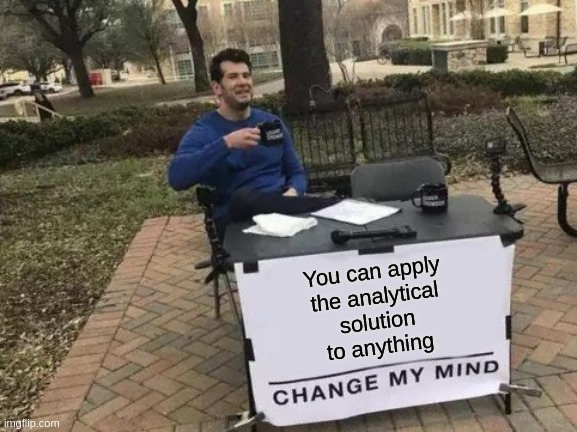
\includegraphics[width=0.3\textwidth]{img/meme_analytical}
    \end{center}
	
\end{frame}
}

\subsection{The need for gradient-based optimization}


\begin{frame}


\notesonly{
We have some cost function we want to minimize but solving the problem analytically is not applicable.

}



\question{In what case(s) do we avoid an analytical solution?}

\pause
\begin{itemize}
	\item We cannot fit all the data into memory.
	\item \notesonly{It involves finding an inverse of a matrix, that is not invertible (e.g. linear regression $(\vec X \, \vec X^\top)^{-1}\vec X \, \vec y_{True}^\top$.
	}
    \slidesonly{
    $$
    \vec w^{*} = (\vec X \, \vec X^\top)^{-1}\vec X \, \vec y_{True}^\top
    $$
    \pause
    but $\vec X \, \vec X^\top$ is not invertible
    }
    \item \notesonly{There is no closed-form solution for the model we're using (e.g. MLP)}
    \slidesonly{no closed-form solution for our model (e.g. MLP with non-linearities)}
	\item Computing the Hessian is too costly. Newton's method also not applicable.\notesonly{\footnote{
	Newton's method finds the root of a function iteratively using the second-order Taylor expansion of the cost function around a point $\vec w_t$. For more details see Haykin Ch. 3.3.
	}}
	\item Non-stationary data. We cannot easily adapt to changes over time.
\end{itemize}

\end{frame}

\mode<article>{

We therefore opt for Gradient-based optimization which is an iterative optimization procedure. 
In the case of a \emph{minimization} problem one can reduce some cost function $E^T_{[\vec w]}$ by taking steps in the direction of steepest \emph{descent}.
For minimizing some cost function $E^T_{[\vec w]}$ w.r.t. to a set of weights $\vec w$, it follows that, if
}
\begin{frame}\frametitle{Alternative: iterative gradient-based optimization}
\begin{equation}
\vec w_{t+1} = \vec w_t - \underbrace{\eta_t \, \frac{\partial E^T}{\partial \vec w} \Bigg|_{\vec w_t}}_{\text{update}~\Delta \vec w}
\end{equation}
\notesonly{
and a small enough }\slidesonly{with }$\eta_t \in \R^+$, then \notesonly{the cost at the next step $t+1$ will become less or remain unchanged. That is} $E^T_{[\vec w_{t+1}]} \le E^T_{[\vec w_{t}]}$.

\mode<article>{
We refer to $\eta_t$ as the learning rate. It allows us to control the size of the step we take in the direction of the gradient.
\emph{Subtracting} the gradient from the current $\vec w_t$ lets us move against the slope in towards some minimum. 
}
\pause
The behavior of gradient descent can be controlled by modulating 
\begin{itemize}
\item The ``scope'' of the gradient. What do we use for deciding on the direction of the update?
\item The learning rate schedule. How big of a step do we take in the direction of the gradient?
\end{itemize}


\end{frame}

\subsection{``Scope'' of the gradient}

\begin{frame}\frametitle{\subsecname}
\mode<article>{
The scope of the gradient method refers to the amount of data used for deciding on the direction of the gradient.
}
\slidesonly{\vspace{-2mm}}
\renewcommand*{\arraystretch}{1.}{
\begin{table}[h]
\begin{tabular}[c]{r|l|l}
\hline
batch      & 
$\displaystyle
\frac{\partial E^{T}}{\partial \vec w} 
\;=\;
\frac{1}{p} \sum_{\alpha=1}^{p} 
\frac{\partial e^{(\alpha)}}{\partial \vec w}
$ &
\pause
\\[10mm]
\hline
mini-batch & \begin{tabular}[c]{@{}c@{}}
$\displaystyle
\frac{\partial E^{T}}{\partial \vec w} 
\;\approx\;
\frac{1}{|\mathcal{M}|} \sum_{\beta \in \mathcal{M}}^{|\mathcal{M}|} 
\frac{\partial e^{(\beta)}}{\partial \vec w}
$\\
$|\mathcal{M}| \ll p$\\
where $\mathcal{M}$ is a set of indices\\
 sampled randomly \\
 from 
 $\{1,\ldots,p\}$
\end{tabular} 
&
\begin{tabular}[c]{@{}l@{}}
noisy \\
estimate of $E^T$, \\
becomes less noisy with \\
larger $|\mathcal{M}|$
\end{tabular} 
\pause
\\[10mm]
\hline
online     &
\begin{tabular}[c]{@{}c@{}}
$\displaystyle
\frac{\partial E^{T}}{\partial \vec w} 
\;\approx\;
\frac{\partial e^{(\beta)}}{\partial \vec w}
$\\
a single random\\ data point $(\vec x^{(\beta)}, \vec y_T^{(\beta)})$
\end{tabular}    &
\begin{tabular}[c]{@{}l@{}}
very noisy \\
estimate of $E^T$
\end{tabular}\\
\end{tabular}
\end{table}
}
\pause
\slidesonly{\vspace{-5mm}}
\question{Which of these can handle non-stationary data?}

\end{frame}

\subsection{Learning rate schedules}

\begin{frame}\frametitle{Robinns \& Munro condition}

\begin{figure}[ht]
     \centering
     \savebox{\imagebox}{
	 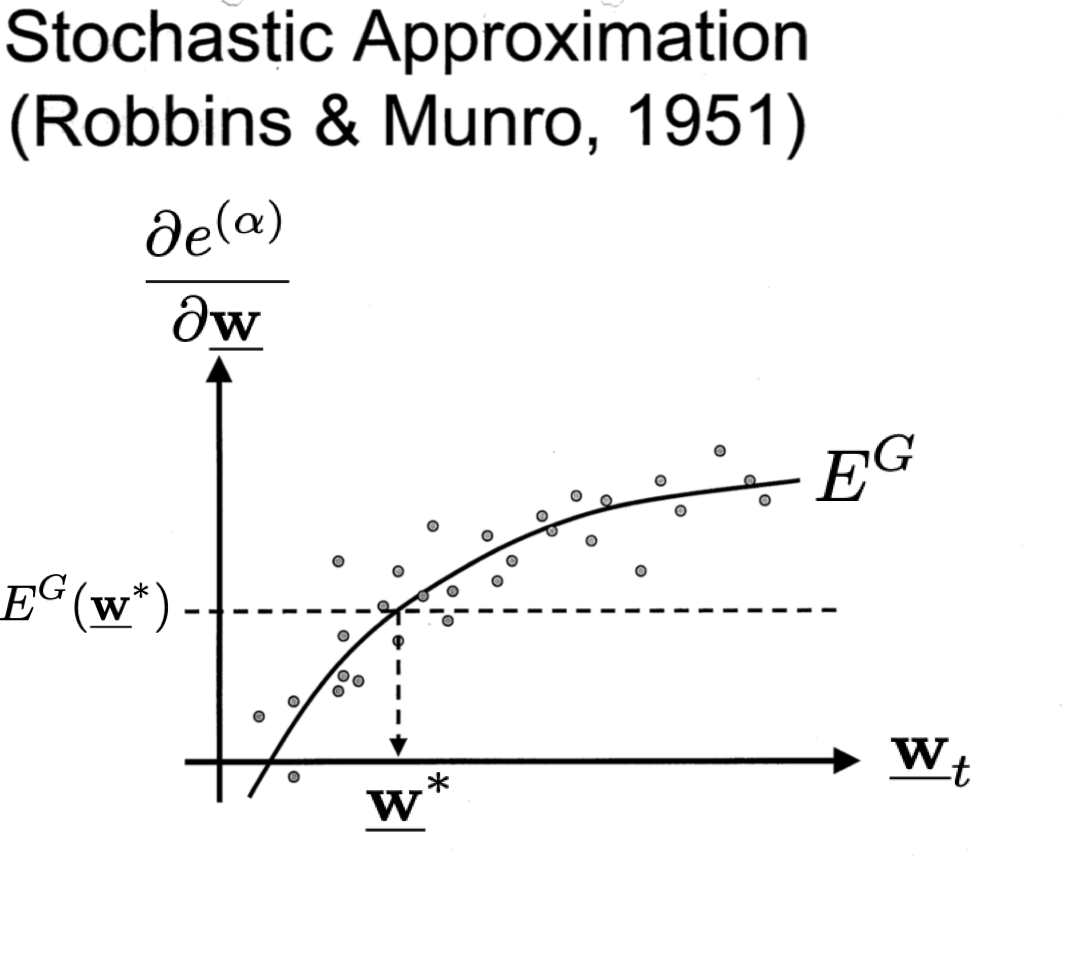
\includegraphics[width=0.5\textwidth]{img/RobbinsMunroNew.png}}%
     \begin{subfigure}[t]{0.35\textwidth}
         \centering
         \usebox{\imagebox}% Place largest image
         \notesonly{\caption{}}
     \end{subfigure}
     \hspace{10mm}
     \begin{subfigure}[t]{0.5\textwidth}
         \centering
         \raisebox{\dimexpr.5\ht\imagebox-.5\height}{% Raise smaller image into place
         \only<2>{
         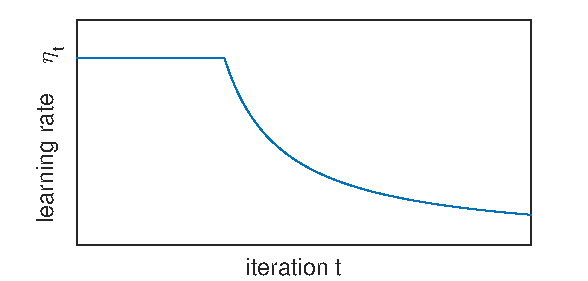
\includegraphics[width=0.99\textwidth]{img/learning_rate-eps-converted-to}
         }
         }
         \notesonly{\caption{}}
     \end{subfigure}
\end{figure}

    
\end{frame}

\begin{frame} \frametitle{Impulse terms}
\mode<article>{
\underline{Impulse terms}:

}
	%\visible<2>{
		\begin{equation*}
			\Delta \vec{w}_{t + 1} \quad=\quad 
			{\color{blue} -{\eta} \frac{\partial E^T}{
				\partial \vec{w}} \bigg|_{\vec{w}_t} } + \;\;
				\underbrace{{\color{red} \mu \; \Delta \vec{w}_t} }_{
					\substack{\text{impulse} \\
						\text{term}}}
		\end{equation*}
	%}
	\vspace{-2cm}
	\only<1>{	
		\begin{center} 
			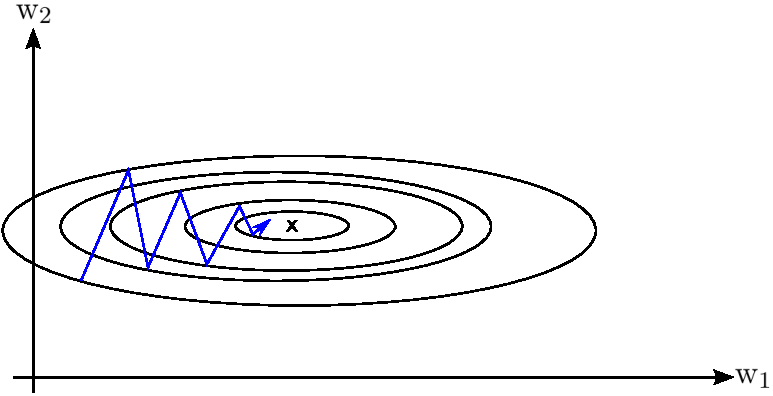
\includegraphics[height=6cm]{img/section1_fig23_clean.pdf} \\
		\end{center}
	} \only<2>{
		\begin{center} 
			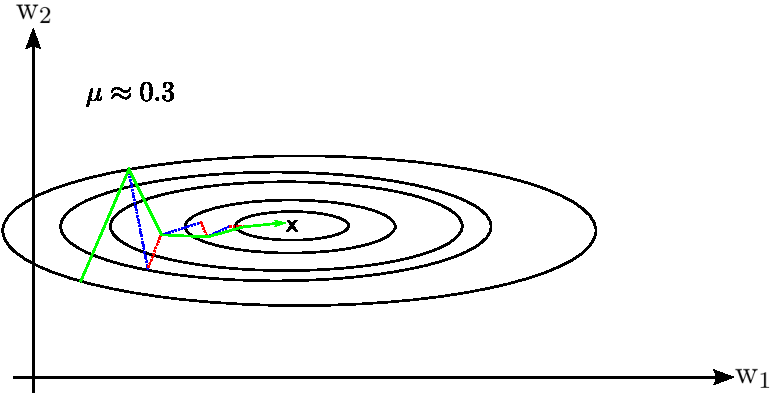
\includegraphics[height=6cm]{img/section1_fig24_clean.pdf}  \\
		\end{center}
	}
\end{frame}

% -----------------------------------------------------------------------------
\begin{frame} \frametitle{Adaptive step size}
 \mode<article>{
\underline{Adaptive step size}:

}   
\begin{center} 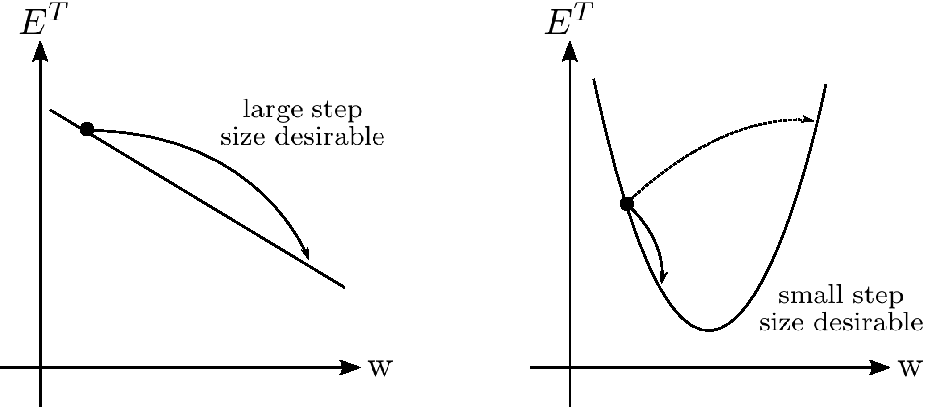
\includegraphics[height=4cm]{img/section1_fig25.pdf} \end{center}
\[ \eta_{t + 1} = \left \{ 
	\begin{array}{lll}
		\rho \eta_t, 
			& \text{if } \Delta E^T < 0,
			& \text{increase step size, if } E^T \downarrow \\
		\delta \eta_t, 
			& \text{if } \Delta E^T > 0,
			& \text{decrease step size, if } E^T \uparrow 
	\end{array} \right.
\]
typical values: $\rho = 1.1, \delta = 0.5$
\end{frame}

% -----------------------------------------------------------------------------
\begin{frame}\frametitle{Line search}
\mode<article>{
\underline{Line search}:

}
   \begin{figure}[h]
    \centering   
    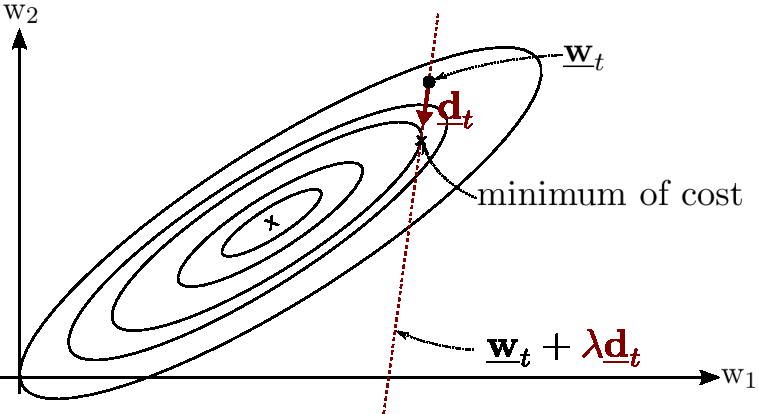
\includegraphics[height=5cm]{img/section1_fig26}
    \mode<article>{
    \caption{Line Search}
    }
    \end{figure}
\end{frame}

\begin{frame}\frametitle{Parabolic interpolation}
\slidesonly{
	\only<1->{\placeimage{9.5}{1}{img/section1_fig26}{width=5cm}}
    \vspace{20mm}
    }
	\begin{center} 
		\includegraphics<1>[height=5cm]{img/parabolicInterpolation_clean_a.pdf} 
		\includegraphics<2>[height=5cm]{img/parabolicInterpolation_clean_b.pdf} 
	\end{center}
\end{frame}


% -----------------------------------------------------------------------------
\begin{frame}\frametitle{Line search}
	\begin{block}{Line search: successive parabolic interpolation}
		\textbf{Initialization:} $a_0, b_0, c_0 \, (\text{on } 
			\vec w_t + \lambda \vec{d}_t);\quad E_{(a_0)}^T,
				\quad E_{(b_0)}^T > E_{(c_0)}^T$
		\vspace{3mm} 

		\While{stopping criterion not fulfilled}{
			\vspace{2mm}
			Fit a parabola through the three points $a_t, b_t, c_t$ \\[2mm]
			Calculate location $d_t$ of its minimum\\[0mm]
			Set $c_{t+1} = d_t,\quad b_{t+1} = c_t,\quad a_{t+1} = \left \{ 
			  \begin{array}{ll}
			 		a_t, & E_{(a_t)}^T < E_{(b_t)}^T \\
			 		b_t, & \text{else}
			 	\end{array} \right.$ 
		}
	\end{block}

	{\scriptsize For details and implementation see 
	e.g.~Numerical Recipes, 2nd edition, Chapter 10.2.}
\end{frame}

\begin{frame}\frametitle{Line search}

\mode<presentation>{
    \begin{center} 
		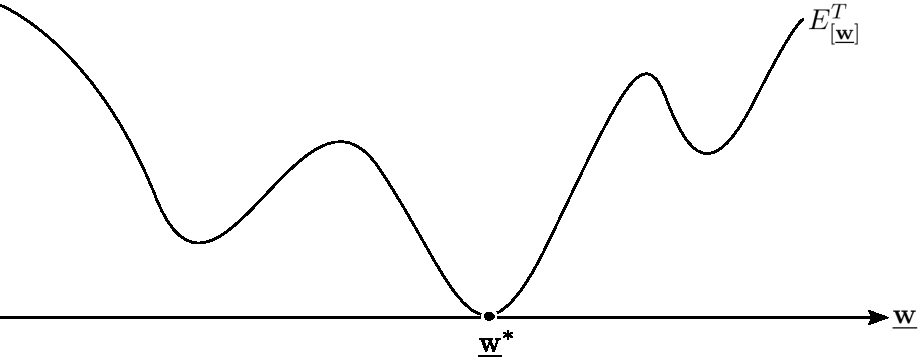
\includegraphics[height=5cm]{img/section1_fig19_no_steps} 
	\end{center}
}

\question{What are potential pitfalls of parabolic interpolation?}

\end{frame}

\begin{frame}\frametitle{Parabolic interpolation}

\mode<presentation>{
    \begin{center}
		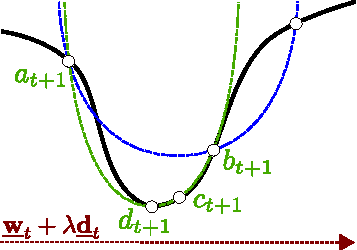
\includegraphics[height=5cm]{img/parabolicInterpolation_clean_b} 
	\end{center}
}

Compute optimal step size:

\begin{equation}
	  \vec{w}_{t+1} = \vec{w}_t - \eta_{t} \vec{g}_t,
	  \qquad \text{with optimal step size} \qquad
	  \eta_{t} = \frac{\vec{g}_t^\top\vec{g}_t}{\vec{g}_t^\top\vec{H}\,\vec{g}_t} \,.
\end{equation}

\end{frame}
